%!TEX root = ../data-imputation.tex
\section{Results}
\label{sec:results}

In this section, we describe and visualize the results of our experiments. For the visualization we choose to consistently use boxplots for all four experiments/scenarios. These allow us to get a decent impression of the distribution of the results based on quantiles. In a line chart, in contrast, the confidence bands would overlap too much to derive meaningful interpretations. The plots' arrangement from left to right corresponds to the degree of difficulty increasing in this direction. This applies to the missingness patterns (MCAR, MAR, MNAR), each of which gets an own sub-plot, as well as the missingness percentages (small to larger), which are depicted as ticks on the x-axis. To show different effects of imputing categorical or numerical columns, we split the plots horizontally. Because we randomly sample on target column for each data set, there are about $13\%$ categorical ($9$) and $87\%$ numerical ($60$) columns. Respectively, for the second experiment, the horizontal split presents classification and regression downstream tasks, which are also imbalanced: $48$ classification ($\sim70\%$) and $21$ regression tasks ($\sim30\%$).



\subsection{Experiment 1: Imputation Quality}

In this experiment we evaluate the imputation performance of each method when training on complete data.

As described above, our goal was to provide a broad overview of the imputation methods' performance on various data sets. Using randomly sampled target columns on heterogeneous data lead to a wide range of values for their evaluation metric ($F1$/$RMSE$), which makes it difficult to compare. To solve this problem, we split the results in categorical and numerical imputation and compute the rank of each imputation method for every missingness pattern and fraction separately. Since we use six imputation methods, there are six ranks, where rank one is best and rank six the worst. If two or more methods perform equal, we assign the same rank and for methods that failed during training rank six.


\subsubsection{Scenario 1: Training on Complete Data}
\label{sec:results_experiment1_scenario1}

\begin{figure}\centering
    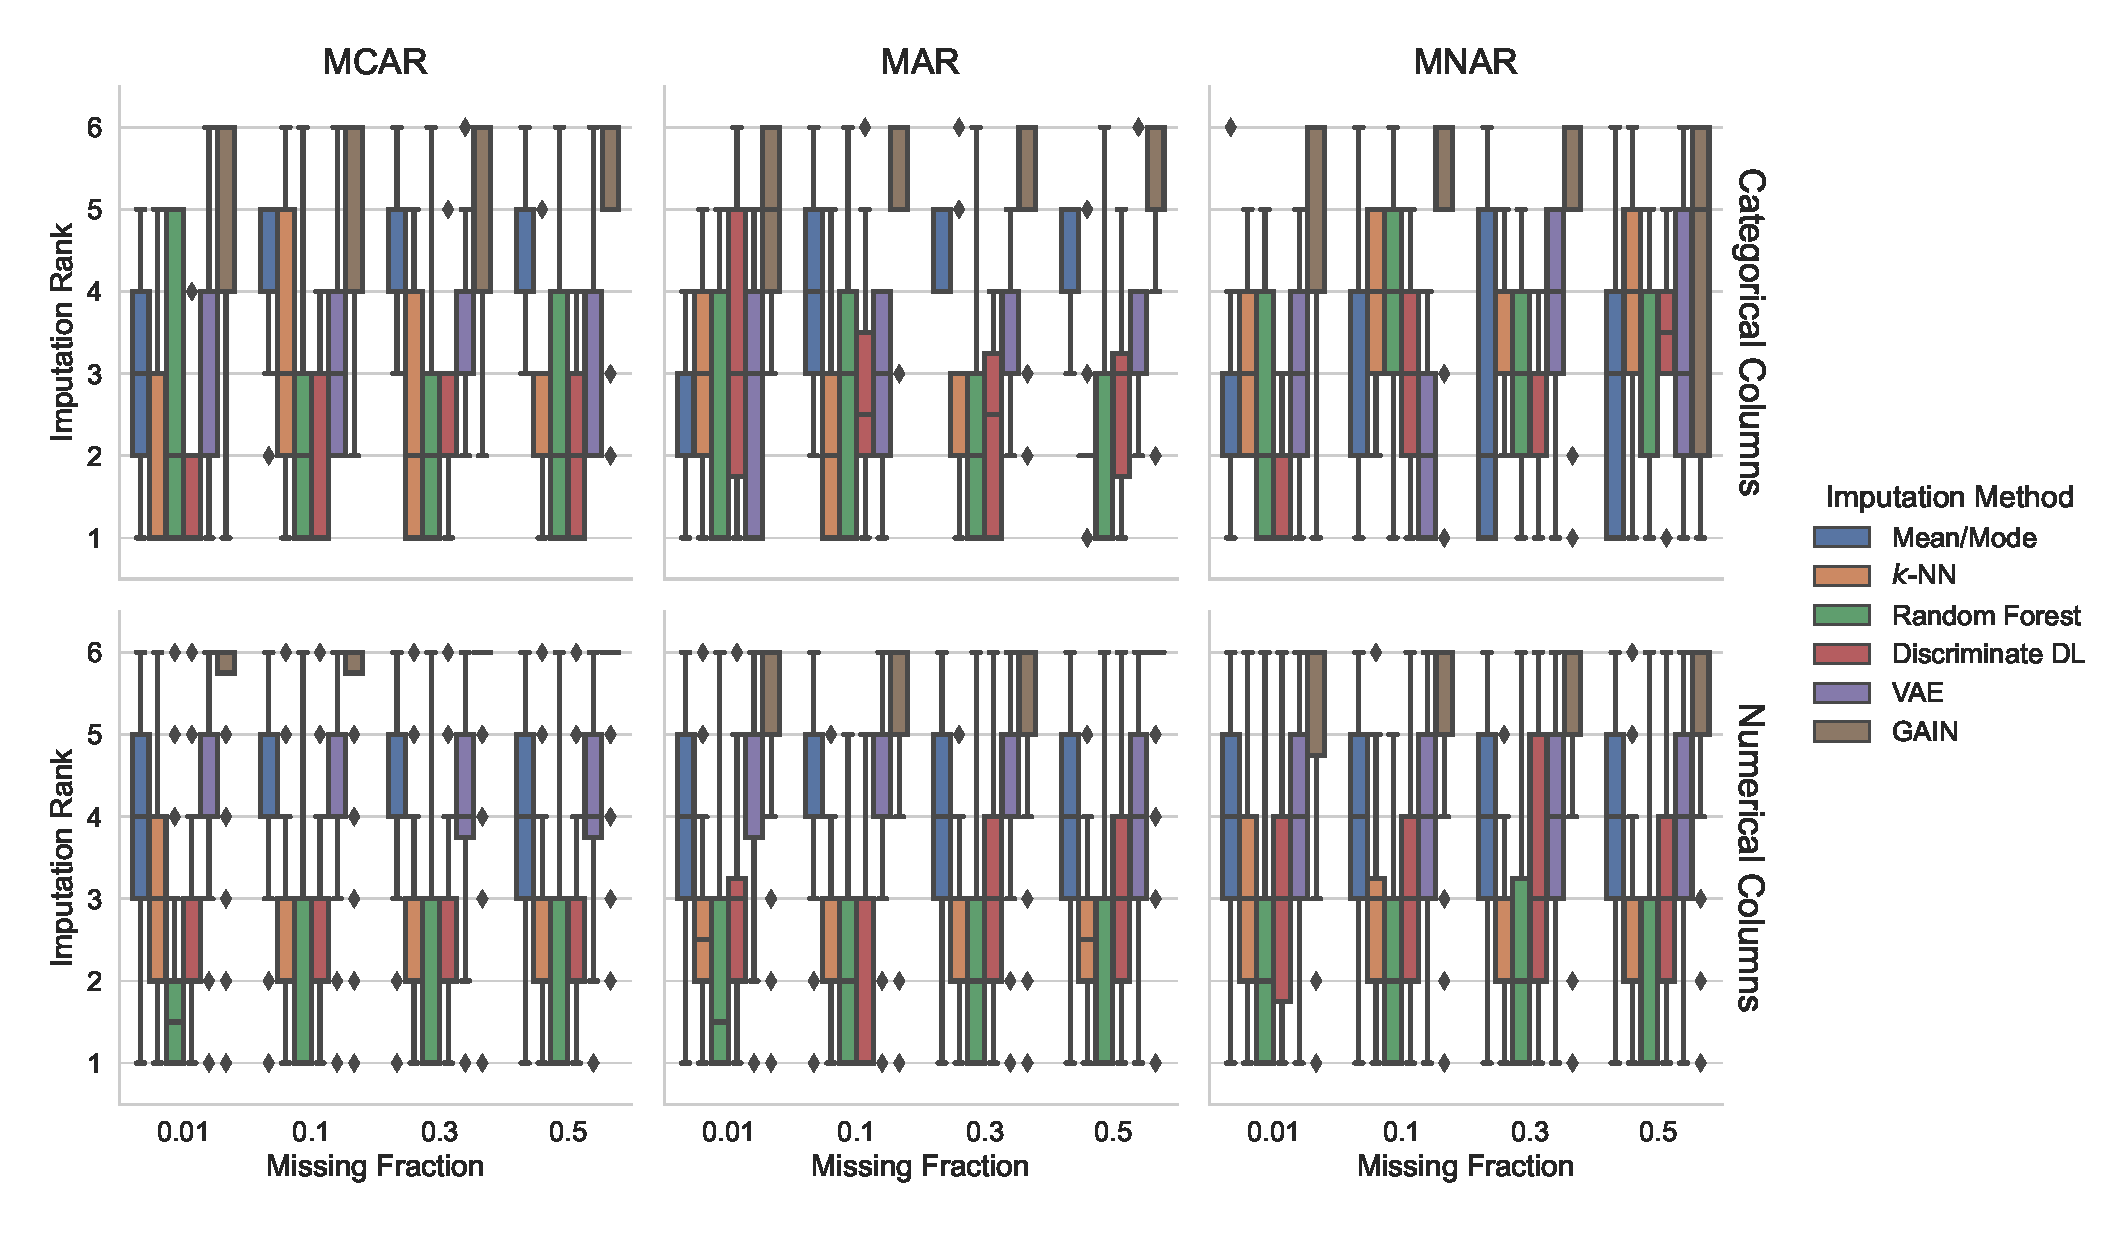
\includegraphics[width=1\columnwidth]{fully_observed_impute_rank_boxplot.eps}
    \caption[Imputation Ranks - Fully Observed]{Imputation ranks of the on complete data trained imputation methods. Ranks are computed for a given experimental setting and range between one and six. The box plots present the distribution of the imputation method's ranks over all cases. Rows distinguish categorical and numerical imputation, and columns the patterns: MCAR, MAR, and MNAR. For numerical imputation, clearly random forest closely followed by $k$-NN and discriminative DL are best. For categorical imputation, the results are less clear. However, the same three tend to be best for MCAR and MAR. For MNAR their performance degrades in favor for mean/mode imputation.
	}
	\label{fig:fully_observed_impute_rank_boxplot}
\end{figure}

%\sebastian{Unterbringen: If an imputation method did not work, it is ranked last. This is most relevant for GAIN, which failed in 273 out of 828 times in \textit{Experiment 1} - \textit{Scenario 1}, which amounts to 33\% of the cases. In \textit{Experiment 1} - \textit{Scenario 2}, however, the problem of GAIN often failing did not occur.}

Figure \ref{fig:fully_observed_impute_rank_boxplot} presents the on complete data trained imputation methods' ranks based on their imputation performance. In about $33\%$ of these results, GAIN failed during training and get assigned the worst rank six.

When imputing categorical columns, there is no clear best method. However, in many settings the discriminative DL approach achieves for $75\%$ of the cases at least rank three or better. Very similar but slightly worse results are shown by the random forest imputation method. For MCAR with $50\%$ missing values and MAR with $10\%$ to $50\%$ missingness, the $k$-NN imputation approach performs good and gets for $75\%$ of the cases at least rank three or better. VAE ranges in most settings for $50\%$ of the cases between rank two and four, and GAIN shows consistently bad performance and ranges in most settings for $75\%$ of the cases on rank four or worse. Interestingly, mean/mode imputation shows better ranks for the more complex settings with MNAR missingness pattern.

When imputing numerical columns the differences are more pronounced. Random forest is the only method that ranges for $75\%$ of the cases among the first three ranks throughout all experimental conditions. Also $k$-NN shows good results, ranging in most settings in $50\%$ of the cases on the second or third rank. Very similar results are shown from the discriminative DL method that tends to lose performance from MAR with $30\%$ missingness to MNAR with $50\%$ missing values. Again VAE ranges most of the time between rank three and five similar to mean/mode imputation and GAIN gets the worst ranks five and six.

To summarize, simple imputation methods, such as $k$-NN and random forest, often perform best, closely followed by the discriminative DL approach. However, for imputing categorical columns with MNAR missing values mean/mode imputation often performs well, especially for high fractions of missing values. The generative approaches get middle ranks (VAE) or range on the worst ranks (GAIN).


\subsubsection{Scenario 2: Training on Incomplete Data}


\begin{figure}\centering
    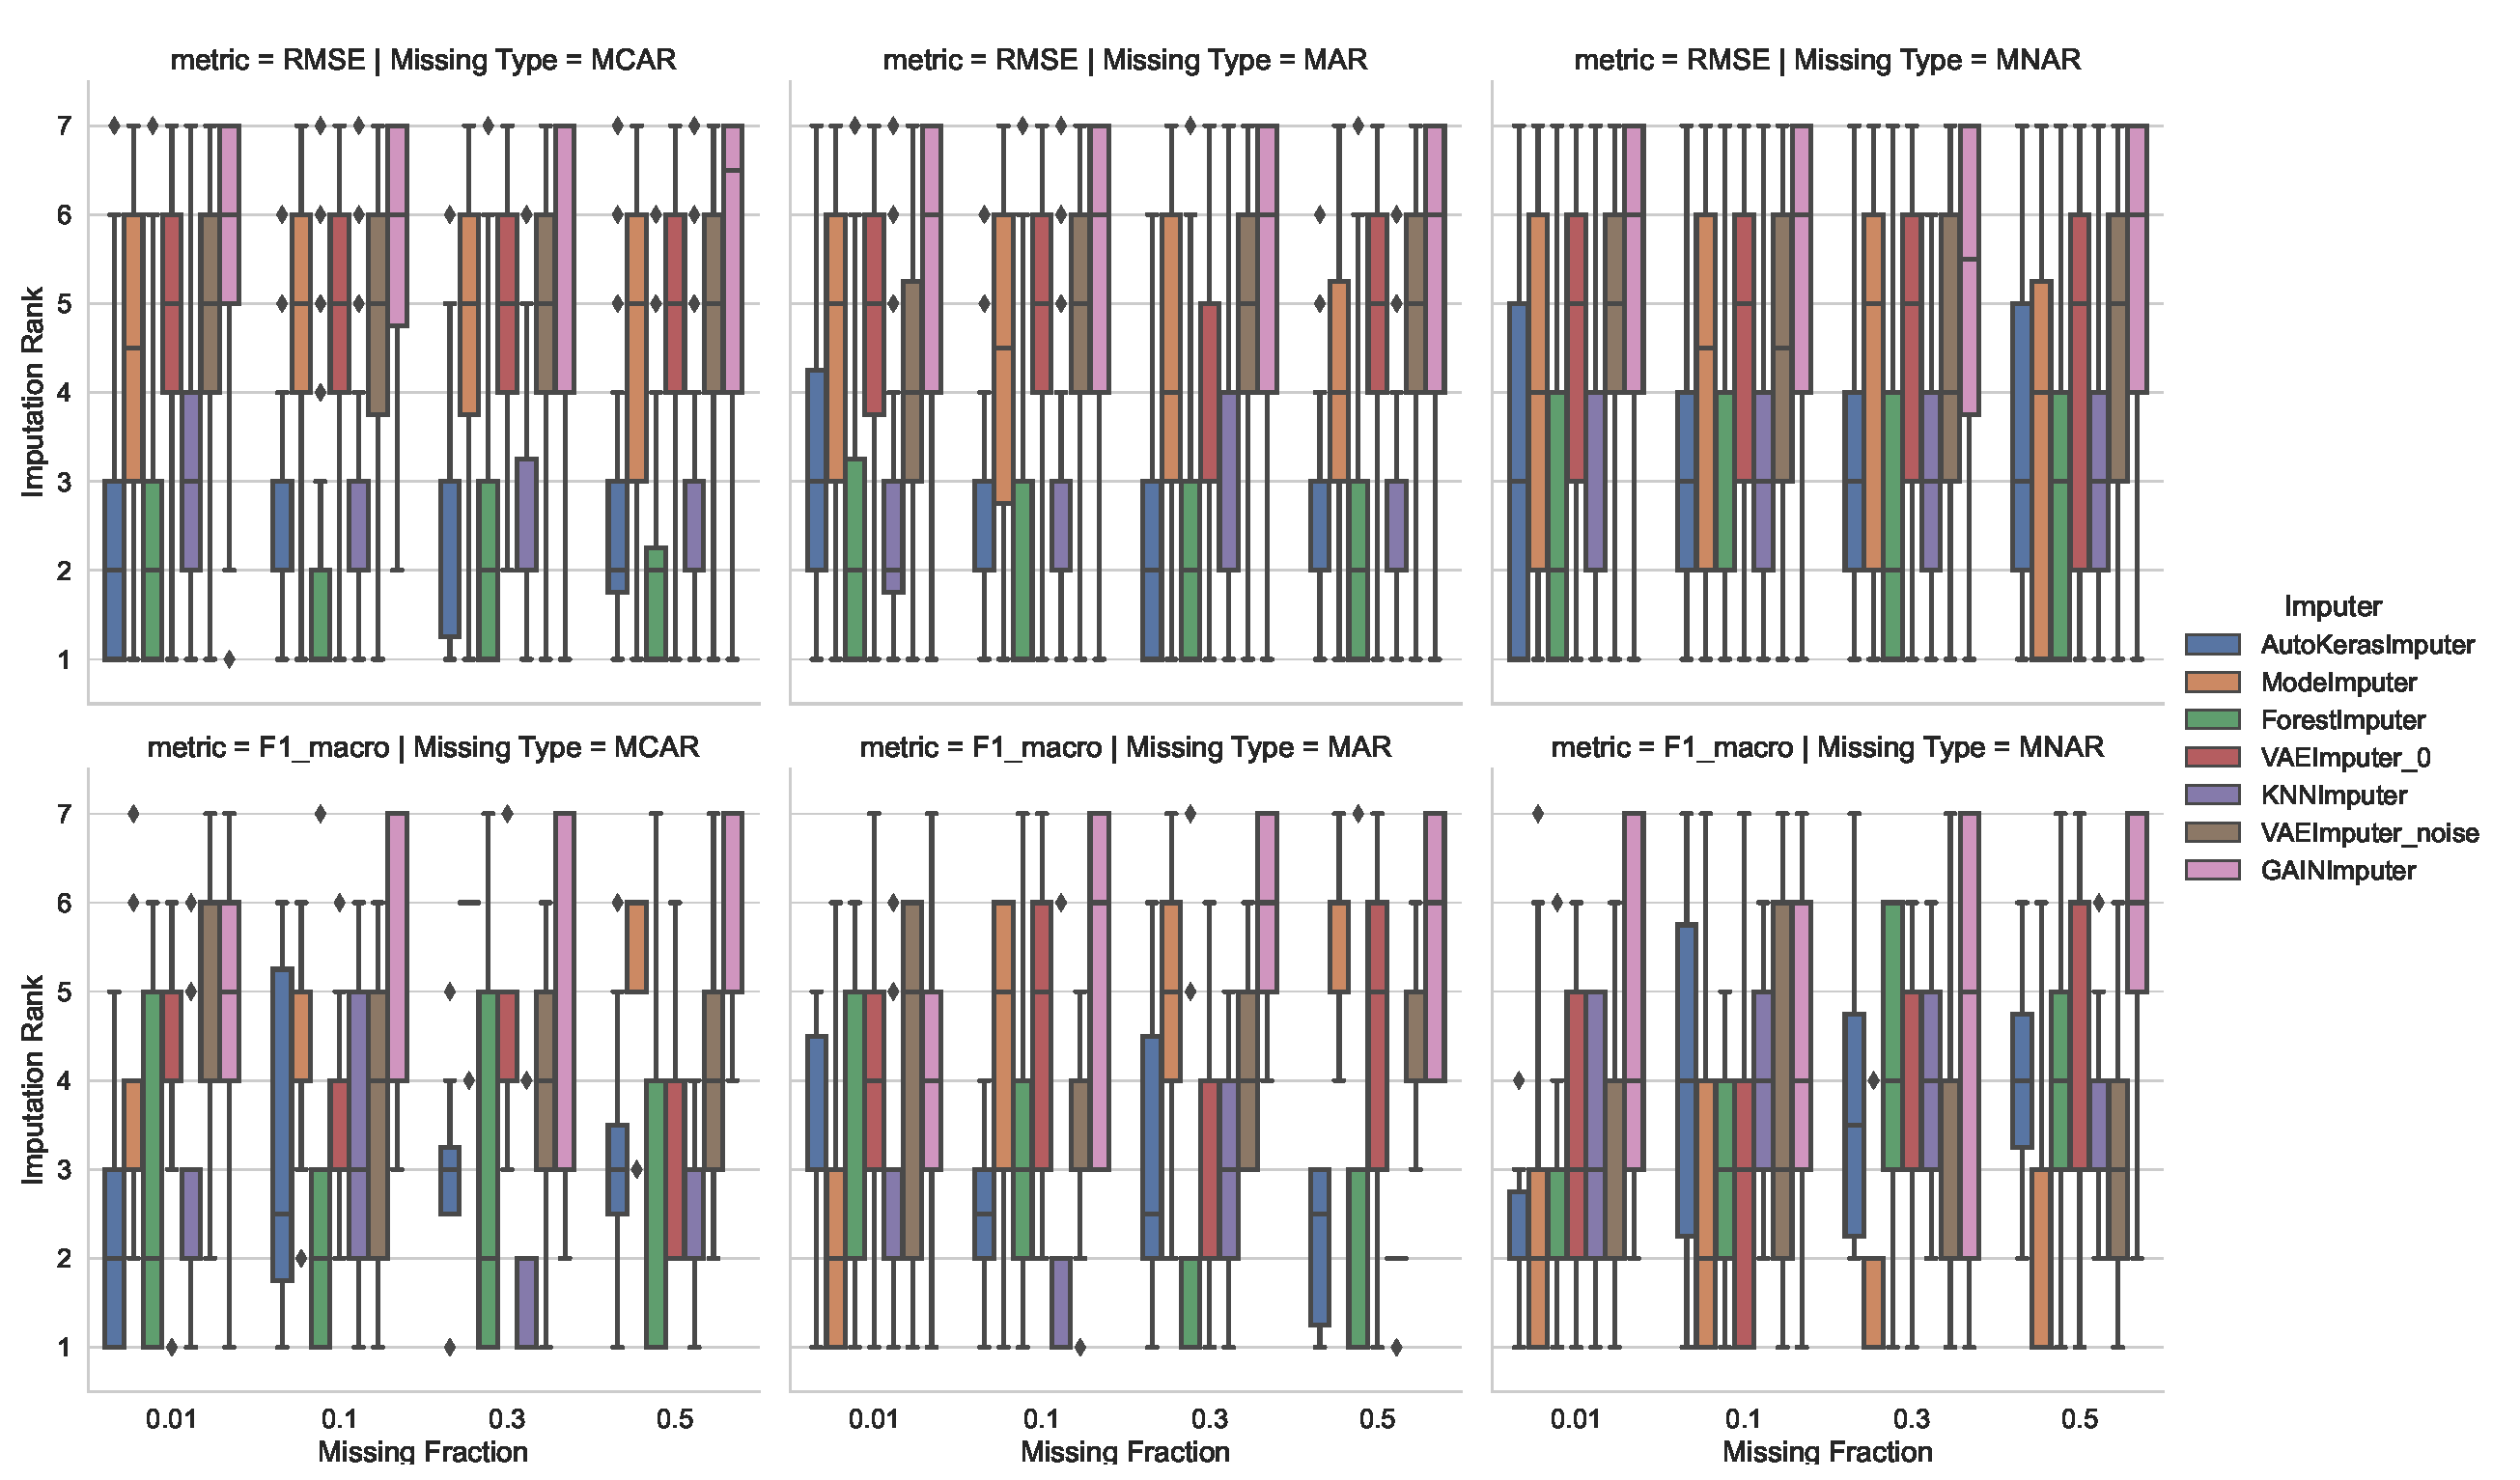
\includegraphics[width=1\columnwidth]{corrupted_impute_rank_boxplot.eps}
    \caption[Imputation Ranks - Corrupted]{Imputation ranks of the on incomplete data trained imputation methods. Ranks are computed for a given experimental setting and range between one and six. The box plots present the distribution of the imputation method's ranks over all cases. Rows distinguish categorical and numerical imputation, and columns the patterns: MCAR, MAR, and MNAR. For numerical imputation, clearly random forest closely followed by $k$-NN and discriminative DL are best. For numerical columns with MCAR and MAR missing values, $k$-NN and random forest are favorable. For MNAR, all approaches degrade in favor of mean/mode that clearly outperforms the other for $30\%$ and $50\%$ missingness.}
	\label{fig:corrupted_impute_rank_boxplot}
\end{figure}

\autoref{fig:corrupted_impute_rank_boxplot} shows the imputation performance in \textit{Scenario 2}, i.e. when training on incomplete data. Imputing categorical columns with increasing difficulty, the ranks of mean/mode imputation improves. From MCAR $30\%$ to MNAR $50\%$, $k$-NN is in $75\%$ of the cases on at least the third rank or better, often it ranges on the first and second rank. For MNAR its performance degrades gradually in favor of mean/mode that show surprinsingly good results, especially for the most challenging settings (MNAR with $30\%$ and $50\%$ missing values) where it clearly outperforms others in at least $75\%$ of the cases. Random forest has very high variance but on most missingness fractions with MCAR pattern, it ranks in $50\%$ of the cases on rank two or better. For MNAR its ranks getting better with higher missingness fractions, whereas this trends reverses for MNAR. The discriminative DL methods shows a very similar trend with tendency to less variance in its ranks. In most cases, the generative methods rank worst (GAIN) and on the middle ranks (VAE). However, with high missingess and when missing values are MNAR, they can perform better.

Similar to the fully observed training case (Section \ref{sec:results_experiment1_scenario1}), imputation on numerical columns yields a clearer ranking than for categorical missing values. The imputation methods $k$-NN and random forest rank best with a tendency of random forest to outperform $k$-NN, where random forest's variance is higher. The discriminative DL approach yields very similar performance to the $k$-NN for MCAR and MAR settings. In the more challenging MNAR setting it ranks slightly worse. For MCAR, mean/mode imputation ranks in almost all settings in $50\%$ of the cases between rank four and five, for MAR and MNAR between rank three and five. Again the generative methods rank in almost all settings in $75\%$ of the cases worse than rank for, where VAE tends to seldom rank the worst rank six.

Overall, the results of \textit{Scenario 1} (Figure \ref{fig:fully_observed_impute_rank_boxplot}) and \textit{Scenario 2} (Figure \ref{fig:corrupted_impute_rank_boxplot}) for numerical columns are quite similar. GAIN has become better in Scenario 2, although it still ranks worst. For categorical the ranks show generally higher variance. Most imputation methods getting worse with higher difficulty of the experimental setting, especially for MNAR, expect of mean/mode, which ranks better for MNAR. This effect is even clearer when training on incomplete data. In general, using simpler methods, such as $k$-NN or random forest achieves good to best results in most settings and cases.


\subsection{Experiment 2: Impact on Downstream Task}

In this experiment we evaluate the downstream performance of each method when training on fully observed data and incomplete data.

In \textit{Scenario 1} we use the definition for \textit{impact on downstream task} from \autoref{eq:impact}. In contrast, for \textit{Scenario 2} we use the slightly different definition from \autoref{eq:impact_scenario2}. Both of theses metrics are labeled \textit{Improvement} and the values represented on the y-axis in \autoref{fig:fully_observed_downstream_boxplot} and \autoref{fig:corrupted_downstream_boxplot}. \felix{Da fehlt was oder? Am besten beschreiben, was geplottet ist, ohne dass man andere definitions nachlesen muss.}

In this experiment, we group the graphs by the type of downstream task. That is, in contrast to \textit{Experiment 1}, irrespective of the data type of the column that was imputed.

Experiemental settings that caused undefined results in the first experiment were filtered out in the second experiment. This means in particular that we have fewer results for GAIN in \textit{Scenario 1}.

When interpreting the results, it should be taken into account that, as described previously (Section \ref{sec:experiment_2}), we only imputed values in the test sets’ target column \felix{die target column der imputation ist nicht die target column des downstream tasks oder? das sollten wir klar trennen.} and measured the downstream improvement based on this.


\subsubsection{Scenario 1: Training on Complete Data}

\sebastian{GANZ WICHTIG: wir haben hier keine infos darüber, welche columns imputed wurden. Was wir sehen ist ne Gruppierung nach Downstream task!}
\arndt{@Sebastian: OK, habs oben eingefügt. Das gilt allgemein für Experiment 2, oder? War mir ehrlich gesagt nicht so richtig klar bisher. Da müssen wir beim Korrekturlesen nochmal drauf achten, dass das nicht irgendwo verdreht ist.}

\begin{figure}\centering
	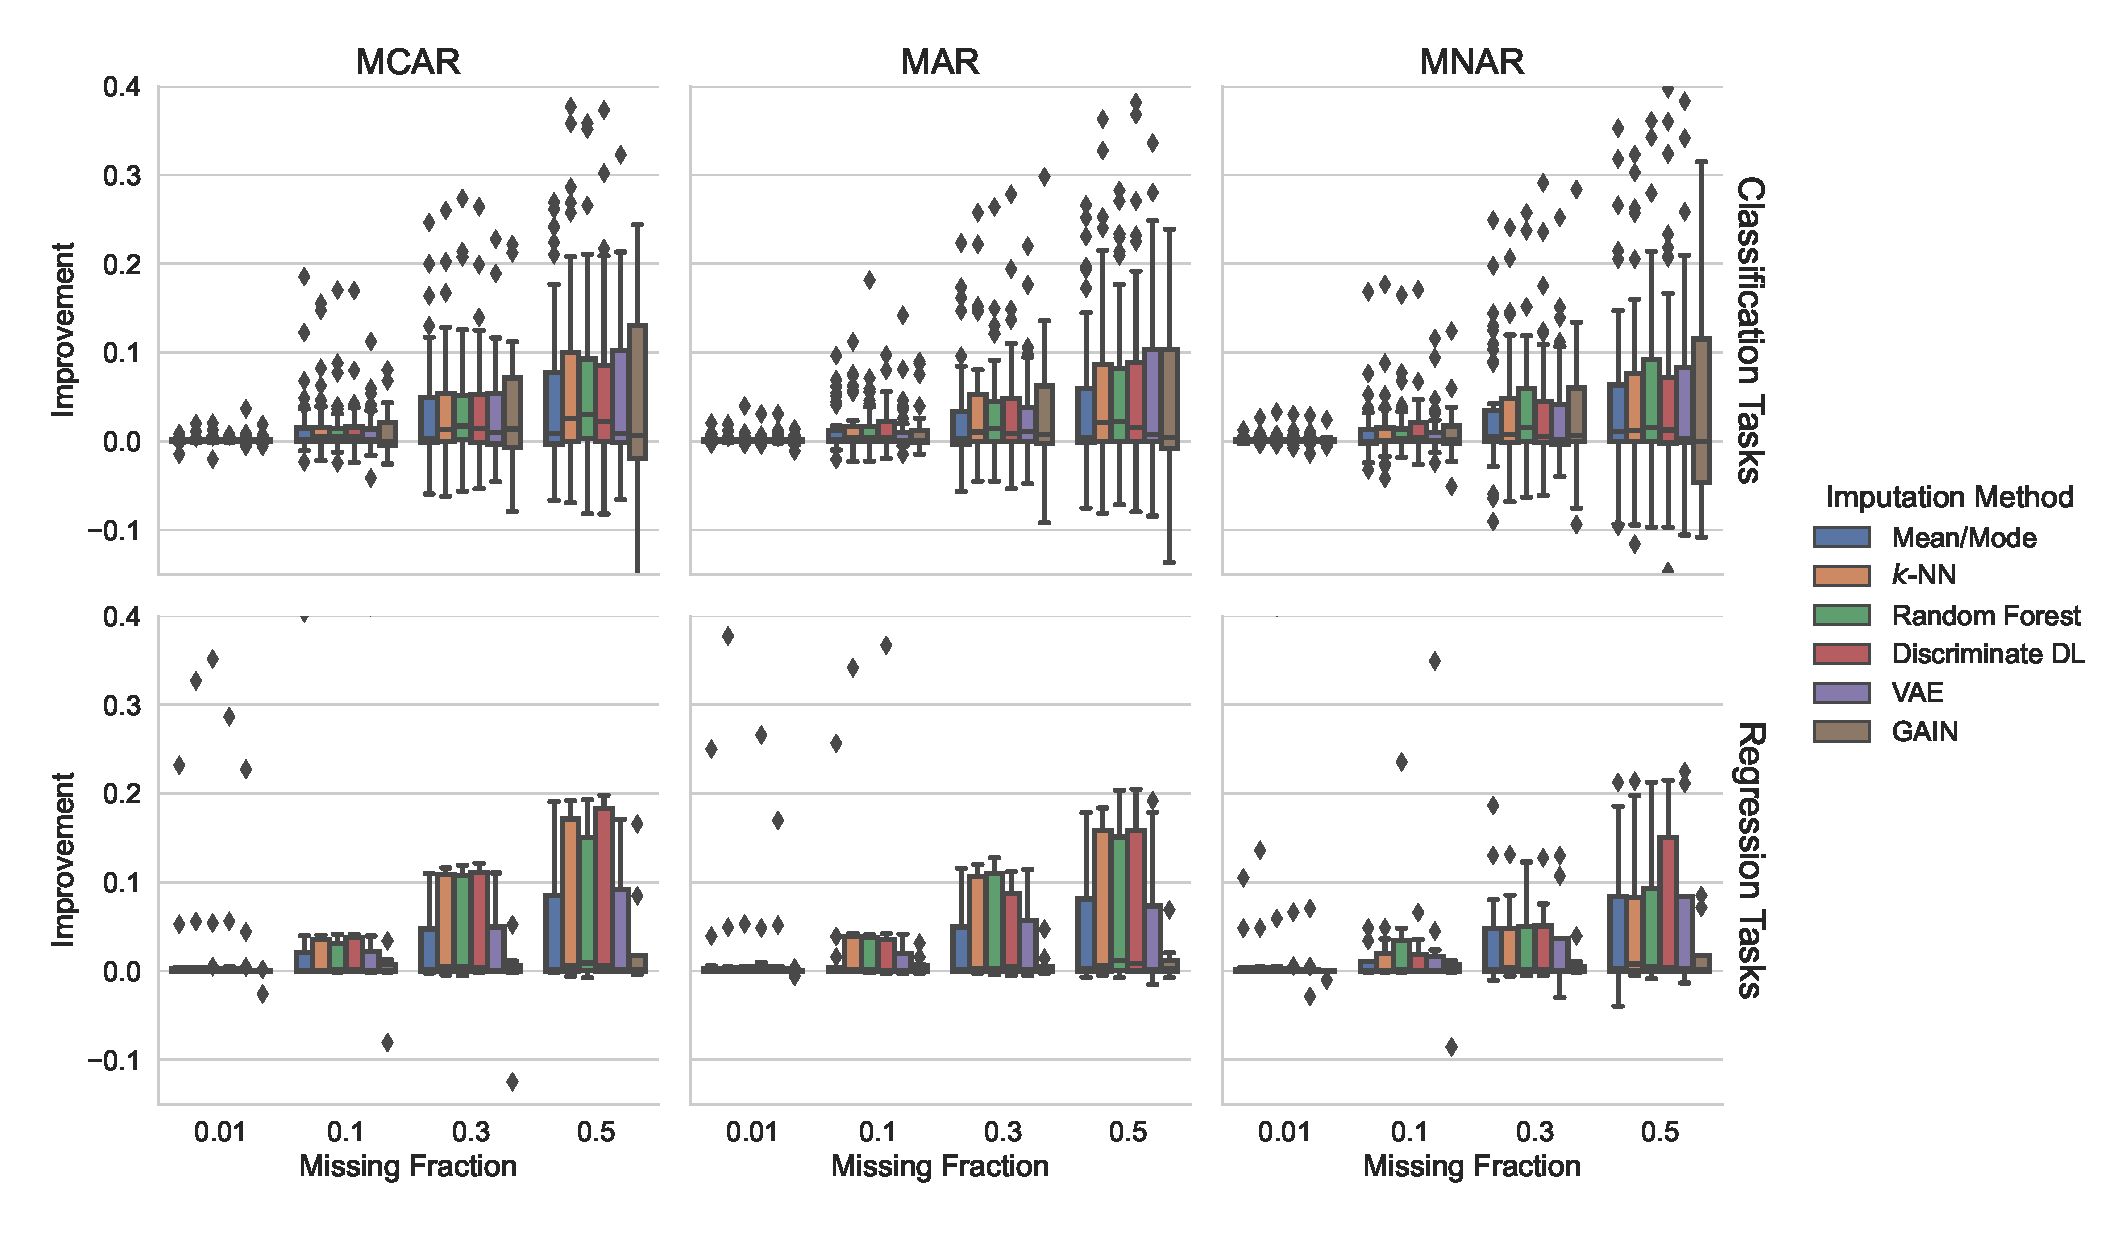
\includegraphics[width=1\columnwidth]{fully_observed_downstream_boxplot.eps}

	\caption[Downstream Ranks - Fully Observed]{Impact on downstream task of the six imputation methods trained on complete data. We plot the imputation method's rank against the missingness fraction. The columns of plots separate the changing missingness pattern, whereas the rows distinguish the results between categorical and numerical target columns. Overall, the classical ML methods and discriminative DL perform best.
    }
	\label{fig:fully_observed_downstream_boxplot}
\end{figure}

Figure \ref{fig:fully_observed_downstream_boxplot} visualizes the \textit{impact on downstream task} metric, i.e. the percent change of the imputation over the incomplete data relative to the baseline (Equation \ref{eq:impact}), in \textit{Scenario 1}.
\felix{Ich wuerde versuchen, das immer so zu beschreiben, dass man es auch ohne andere definitionen verstehen kann, also etwa: percent change of the imputation over the incomplete data relative to the downstream task performance on fully observed data }

\felix{das deutlichste ergebnis ist: imputation hilft! das sollte man auch genauer beschreiben, also etwa: in many conditions imputation improves the downstream performance by XY\%}
The impact of imputation seems mostly negligible if the proportion of missing values is only 1\%. However, for numeric columns, there are some outliers in the 20\% to 40\% improvement range with the MCAR and MAR patterns at 1\% missing values. With an increasing proportion of missing values we observe increasing improvements in the downstream performance in all types of missingness patterns. However, there are also some cases where downstream performance is degraded by imputation, which is mainly the case for categorical columns. \felix{das kann man auch quantifizieren, es sind ja weniger als 25\% der Faelle.}

For categorical columns, improvements are mostly in the 0\% to 5\% range, and in case of 50\% missing values the upper quartile reaches the 5\% to 10\% range. The whiskers even indicate performance increases which go significantly beyond. Measured by the median, as an overall aggregation, random forest yields the best results for categorical columns. GAIN performs often similarly well or even better but also has more negative fluctuations.

\felix{die unterschiede zwischen den Methoden sind nicht sehr deutlich, man kann die beschreibung dabei belassen, dass es keine richtigen unterschiede gab, denke ich.}
The situation is different for regression tasks. Here, GAIN clearly yields the least improvements downstream. Even the Mean imputation is oftentimes significantly more beneficial for the downstream tasks. The VAE results are approximately on par with Mean imputation. In contrast, the classical ML and the discriminative DL approaches do outperform the other methods in most settings. However, when the missing values are MNAR there is no clear advantage except that the discriminative DL is superior at 50\% missing values.

Overall, the classical ML methods and discriminative DL perform best. Again, mean/mode imputation yields medium good results. As the proportion of missing values increases, we observe increasing improvements of the in downstream performance in all types of missingness patterns, along with higher variance. In contrast to classification tasks, there are hardly any negative effects in regression tasks.


\subsubsection{Scenario 2: Training on Incomplete Data}

\begin{figure}\centering
	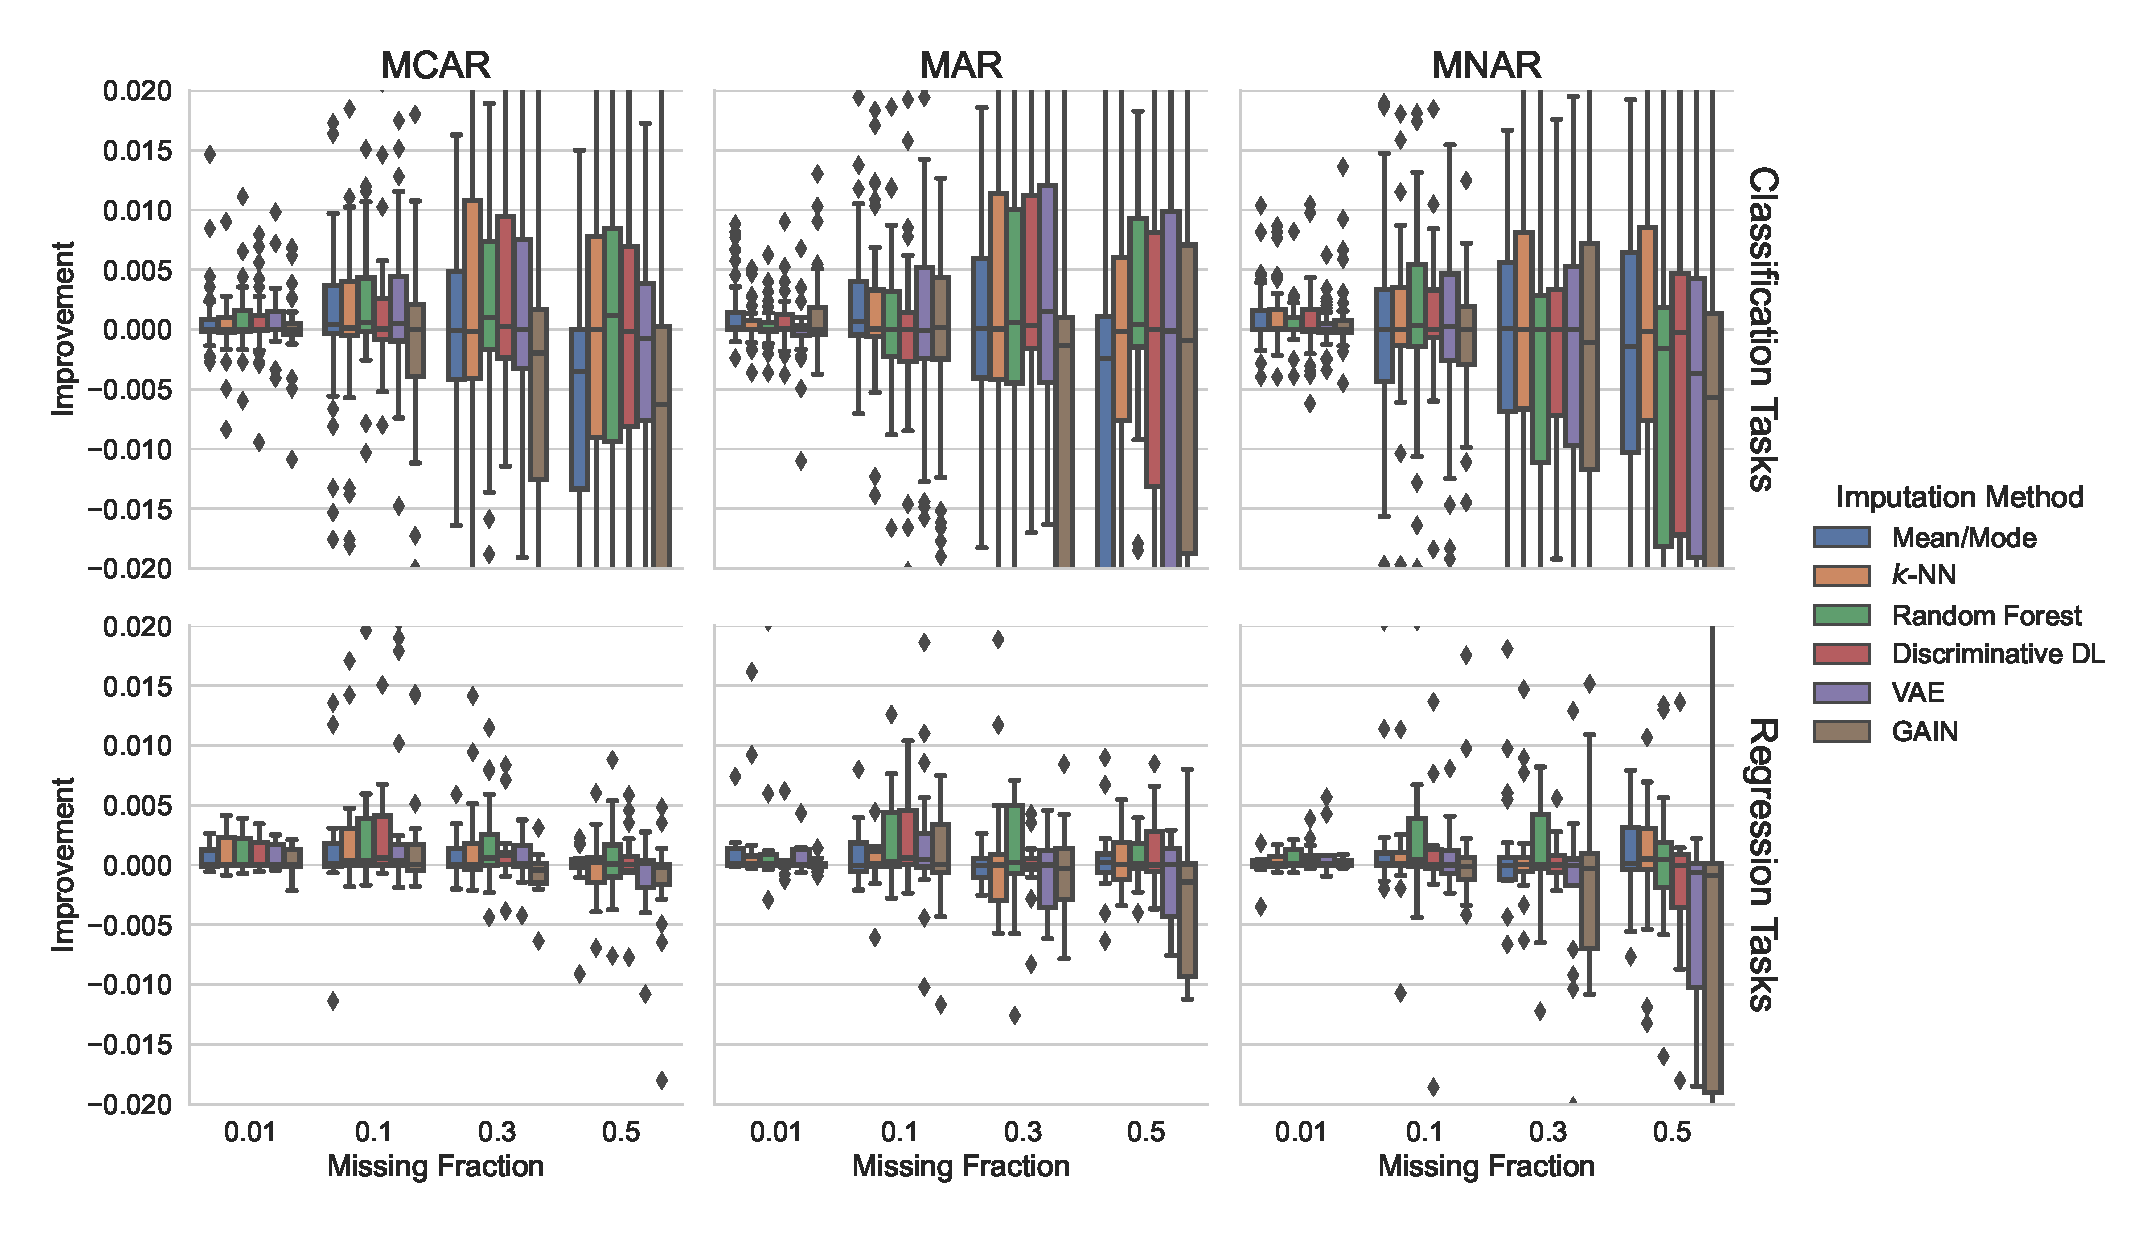
\includegraphics[width=1\columnwidth]{corrupted_downstream_boxplot.eps}

	\caption[Downstream Ranks - Corrupted]{Impact on downstream task of the six imputation methods trained on incomplete data. We plot the imputation method's rank against the missingness fraction. The columns of plots separate the changing missingness pattern, whereas the rows distinguish the results between categorical and numerical target columns. In regression tasks, no considerable improvements are achieved. In classification tasks, in contrast, we observe slightly positive effects in some settings but negative effects predominate in the harder settings.
    }
	\label{fig:corrupted_downstream_boxplot}
\end{figure}

Figure \ref{fig:corrupted_downstream_boxplot} illustrates the \textit{impact on downstream task} (Equation \ref{eq:impact_scenario2}) in \textit{Scenario 2} (training on incomplete/imputed data). Here, the different scaling of the y-axis must be taken into account, i.e. the relative improvements are significantly smaller compared to the first scenario. One reason for this is the different basis for calculating the relative values (see sections \ref{sec:experiment_2} and \ref{sec:scenario_2}).

If weak positive effects seem to predominate in classification tasks at first, this tendency changes with increasing proportion of missing values (at 50\%) and increasing difficulty of the task (especially MNAR). The most negative results are produced by GAIN. However, the other methods also have major difficulties and often drift into negative ranges for the greater part as the tasks become more challenging.

In regression tasks, apart from a few outliers, there are no significant improvements. At the highest proportion of missing values (50\%) and greatest difficulty (MNAR), the results of the generative methods (VAE and GAIN) even turn predominantly negative.

Here, too, the variance increases with higher fraciton. However, this time the results tend to worsen. In summary, no considerable improvements are achieved in regression tasks. In classification tasks, the picture is more mixed and the variance is higher. In some settings, there are slightly positive effects to note. In the difficult settings, however, the negative effects predominate. Again, $k$-NN and random forest appear to be the most robust methods overall.

\arndt{consider points below in discussion}
\felix{
\begin{itemize}
\item in the conclusion we should relate the performance to the training and prediction time and comment on the (large) differences - for AutoKeras, a lot more tuning is performed and we don't know whether it would have worked as well with less tuning.
\item we should highlight the limitations of our results (only one column, maybe too simple)
\item we should highlight the main findings; as far as i can see this would be: a) classical methods perform best (on these simple (?) data sets) and b) downstream performance is improved by X \% in Y \% of the experiments (we can use the quantiles in the boxplots) whereas when the imputation methods are trained on incomplete data, we cannot expect improvements.
\end{itemize}
}
\sebastian{
\begin{itemize}
\item Scenario 2: Training on Incomplete Data - Spätestens jetzt sollten wir mal ein wort darüber verlieren woran das liegen könnte: When eine category einfach häufiger ist, dann ist das meist ne recht guter guess. Das könnte dazu führen, dass die andere schlechter werden, weil die versuchen das intelligenter zu machen, aber einfach nicht genügend trainings daten haben um noch was sinnvolles zu lernen
\item Figure 3 - (Hbane wir ne idee warum classificaiotn auch schelcht wird und regression nicht?)
\end{itemize}
}

\subsection{Computational Complexity}
%
\sebastian{Add rest experiments + check whether description is still valid}
To measure the training and inference time, we use a sub-set of our experiments. Precisely, all data sets, missingness fractions and imputation methods (shown in Table \ref{tab:experiment_settings}) with MCAR pattern. We first train the imputation method on complete data, then discard values of the given missingness fraction in the training set, and impute those missing values. The wall-time is measured in seconds when calling our framework's \code{fit} and \code{transform} methods (see Section \ref{sec:implementation} for details), which means that the training duration incorporates the hyperparameter optimization (see Section \ref{sec:HPO} for details).

Because training and inference time depend heavily on the data set's size, directly average all experiments for the imputation methods lead to very similar mean but extremely high standard deviation values. For this reason, we first compute the mean duration and the standard deviation relative to its mean separately for training and inference for the imputation methods on each data set. Second, we average those values for each imputation method and present them in Table \ref{tab:time}. Using this approach helps to average over all experiments, and, at the same time, gives indicators for the training and inference durations, as well as their variance.
%
\begin{table}
	\centering
	\begin{tabular}{@{\extracolsep{4pt}}lllll@{}}
		\toprule
		\multirow{2}{*}{Imputation Method} & \multicolumn{2}{c}{Training} & \multicolumn{2}{c}{Inference} \\\cline{2-3}\cline{4-5}
		\\[-0.75em]
		& Mean Duration &   Rel. SD & Mean Duration &   Rel. SD \\
		\midrule
		Mean/Mode &      0.005277 &  0.550878 &      0.029195 &  0.171139 \\
		\\[-0.5em]
		$k$-NN &     41.204365 &  0.253716 &       7.01833 &  0.602026 \\
		\\[-0.5em]
		Random Forest &    226.076551 &  0.119295 &     11.438507 &  0.245989 \\
		\\[-0.5em]
		Discriminative DL &   6275.019244 &   0.40505 &    355.920893 &  0.194171 \\
		\\[-0.5em]
		VAE &     71.095282 &  0.098795 &      9.093325 &  0.084075 \\
		\\[-0.5em]
		GAIN &    878.058286 &  0.311553 &     48.948755 &  0.086431 \\
		\bottomrule
	\end{tabular}
	\caption{Training and inference duration for each imputation method in seconds. We use the wall-time to measure the durations for training, including hyperparameter optimization, and inference for all data sets with MCAR missingness pattern and all fractions shown in Table \ref{tab:experiment_settings}. Because training and inference durations depend heavily on the data set size, we first calculate the durations' mean and relative standard deviation for each imputation method on every data set. Second, we average those mean durations and relative standard deviations for the imputation methods and present them as \emph{Mean Duration} and \emph{Rel. SD} separately for \emph{Training} and \emph{Inference}. Abbreviations: \emph{Rel. SD} means Relative Standard Deviation.}
	\label{tab:time}
\end{table}

Striking but not surprisingly, if the imputation model's complexity increases, their training duration increases too, most of the time by multiple factors. There are two exceptions: discriminative DL and VAE, an explanation for this could be their number of hyperparameter combinations optimized during training. VAE optimizes only three, GAIN $16$, and discriminative DL $50$ combinations, which represents their training durations order.

Similarly, the inference time increases with the model's complexity. The differences are clear but not as high as for the training durations.
Higher inference standard deviations, e.g., for $k$-NN and random forest (and discriminative DL), indicate that the found best hyperparameters strongly varying with the experimental settings and influence the model's computational complexity for inference. One reason for the discriminative DL's and GAIN's high training standard deviations could be the usage of early-stopping and, at the same time, indicate that it is important to try a huge number of hyperparameters to achieve good results. For mean/mode the high standard deviation is likely an artifact of the very small training duration. Changes in milliseconds for computations are common and represent a large change relative to the mean/mode imputation's mean duration.

To summarize, the increasing complexity of the imputation methods are clearly represented in their training and inference duration. For training more complex models, this is supported by higher variance of training time indicating the necessity to try a wide range of hyperparameters. On the other hand, once found, the hyperparameters  for generative models influence the inference time less than for $k$-NN or random forest, which prediction times depend heavily on the hyperparameters.
